%
%                       This is a LaTeX 2e version of the
%                       laboratory project template file.
\documentclass[a4paper,twoside,12pt]{article}
\usepackage{fullpage,epsf}
\usepackage{color,graphicx,natbib}
\usepackage{gensymb}
%\graphicspath{ {C:/Users/Emma/Documents/TU Delft/International Course for Computational Physics} }

% Make subscripts in text available
\DeclareRobustCommand*\textsubscript[1]{%
  \@textsubscript{\selectfont#1}}
\def\@textsubscript#1{%
  {\m\ensuremath{_{\mbox{\fontsize\sf#1}}}}}
%
%                       This section generates a title page
%                       Edit only the sections indicated to put
%                       in the project title, your name, supervisor,
%                       project length in weeks and submission date
%
\begin{document}
\pagestyle{empty}                       							% 	No numbers of title page                      
                                           								% 	Centre Title, and name
\vspace*{2cm}
\begin{center}
        \Large\bf International Course for Computational Physics\\[10pt]% 	Change to MP/CP/Astro
        \LARGE\bf Monte Carlo Cluster Algorithm\\	         		% 	Change to suit
       \bf Ising Model\\
\end{center}
\vspace*{0.5cm}
\begin{center}
        \bf Jason Emming\\ 									% 	Replace with your name
        March 2015                                    						%	Submission Date
\end{center}
\vspace*{5mm}

\vspace*{2cm}
Signature:\hspace*{8cm}Date:

\vfill
{\bf Lecturers:} Dr. Phil Duxbury        					
\hfill
\textbf{Year:} 2014-2015                 					
\newpage
											%      End of Title Page
\pagestyle{plain}                               					% 	Page numbers at bottom
\tableofcontents                                					% 	Makes Table of Contents

\pagebreak

\setcounter{page}{1}                         					% 	Set page number to 1

\section{Introduction}
At a first glance using random numbers to solve physics problems seems strange. However, this is exactly how computer algorithms, such as the Monte Carlo Method work. Often, algorithms such as these are used to solve mathematical problems that are much too difficult using traditional methods. Areas in physics such as protein folding, chemical engineering and analyzing nuclear particle showers all beneficent from the random sampling done in the Monte Carlo Method. The goal of this assignment was to apply this method to the Ising model of ferromagnetism using a cluster algorithm approach and estimate a value for the critical temperature.  


\section{Theory}
In order to accurately model how temperatures affect the magnetization of ferromagnetic materials, we gave each atom certain properties. We modeled each atom as a single cell in an NxN matrix. These cells were each initialized with a certain value for their magnetic spin. The value of the spin and how each cell interacted with its closeted neighbors provided the basis for our program and gave us estimates of the critical temperature for a generalized system.

\subsection{Critical Temperature}
The critical temperature, known as the Curie temperature when discussing a material's intrinsic magnetic properties, is the temperature at which certain kinds of magnetic materials undergo a rapid change in their magnetism. Put a iron magnet inside blacksmith's oven, and you will find it has lost its magnetization. This is because the Curie temperature for iron is \textasciitilde770 degrees Celsius, well within the temperature range needed to smith iron. This critical temperature is characterized by its sudden change in magnetization at a very small temperature range, see figure \ref{fig:Mag}. We define the critical temperature at the point of the magnetization's greatest change. In other words, it is the temperature at which the derivative is largest, see figure \ref{fig:dMdT}. 

\subsection{Ising Model}
The Ising model is a mathematical tool used to understand ferromagnetism. The model is designed so that the magnetic dipole moment of each atomic spin is aligned in one of two directions, up (+1) or down (-1). These spins are laid out in a lattice, so that each spin can interact with its nearest neighbors. In the case of our 2D lattice there are four neighbors for every atom. Modeling these ferromagnetic properties can help us understand why magnets demagnetize when under a specific temperature. 


\section{Computational theory}

\subsection{Cluster Approach}
The cluster approach to the Ising model is unique. Instead of repeatedly choosing a random cell in the lattice and flipping its magnetic spin, we choose a cell and grown a cluster from that location until it can grow no further, we then flip the cluster as a whole. The idea behind this approach is the reduce computation time. 

\vspace{3mm}

\noindent Once a cell has been chosen, using a random number generator, it can grow to its neighbors. In this 2D case, either up, down, left, or right, but first the spin of the neighbor and the chosen cell must be aligned (same value). If this is the case, determining whether it will join the cluster is simply probabilistic. We start by generating another random number, this time between 0 and 1. We compare this number to the value given by equation \ref{eq:prob}. 

\begin{equation}
\label{eq:prob}
P = 1 - e^{\frac{-2J}{k_{B}T}}
\end{equation}

\noindent Where \textit{J} is the ferromagnetic exchange constant, $k_{B}$ is the Boltzmann constant, and \textit{T} is the temperature at which the cluster is being grown at. If the value of \textit{P} is greater than that of the randomly generated number then the cluster will absorb that neighbor. Once a neighbor is added to a cluster all of its immediate neighbors are now eligible to join as well, assuming their spins are also aligned. However, if the value of \textit{P} is less than the random number, then the connection between those two cells is broken and the cluster cannot grow in that direction. 

\vspace{3mm}

\noindent It is important to note that the cluster's growth is dependent on the temperature of the system. At very low temperatures the probably of absorbing neighbors is very high. Therefore, we can expect to generate large clusters at low temperatures and small ones at high temperatures.
Also, in our simulation, both \textit{J} and $k_{B}$ have been set to one. As a consequence the values of the temperatures we graph do not represent units such Kelvin, Celsius, or Fahrenheit.

\subsection{Boundary Conditions}
In our Monte Carlo code we imposed periodic boundary conditions. By doing so, we approximated an infinite system, while only simulating a small unit. Cells on the edge of the lattice were given neighbors from the opposing side and vis versa. This allowed each cell to have four neighbors regardless of the dimensions of the lattice.
This was done very simply by taking the modulo of their position in the lattice. If an atom was in the tenth cell of a 10x10 lattice then it would have an index of 9, as is typical of a computer coding index. Its following neighbor's index would then be ten. Since the indexing on a 10x10 lattice ends at nine, taking the modulo of the neighboring index would always correct for this and apply the appropriate boundary conditions. e.g. 10 mod 10 = 0, see figure \ref{fig:periodic_boundary}.

\begin{figure}
\centering
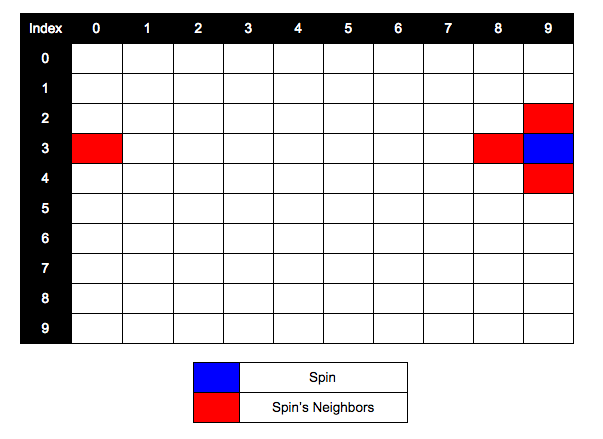
\includegraphics[scale=0.3]{Figures/Lattice_Neighbors.png}
\caption{Periodic boundary conditions of a cell on the edge of the 10x10 lattice, with its neighbors in red.}
\label{fig:periodic_boundary}
\end{figure} 



\section{Results}
Clusters where grown repeatedly on a lattice for each temperature. The amount grown was a function of both the lattice size and the temperature itself. Once the lattice reached an equilibrium point known as its 'steady state', we measured the magnetization and internal energy of the system. We believed this magnetization and energy to be characteristic of the particular temperature being tested. To reduce random errors, we repeated these exact same measurements multiple times and averaged the results.

\subsection{Magnetization}
The magnetization was determined by simply adding up all the spins (+1 or -1) and dividing by the number of cells, $N^2$, to normalize the result.

\begin{figure}[h]
\centering
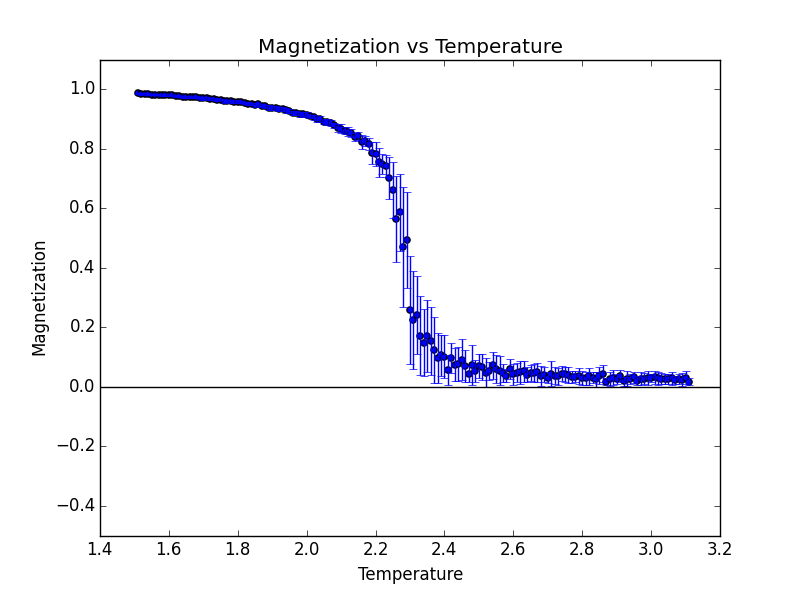
\includegraphics[scale=0.5]{Figures/Mag.png}
\caption{Magnetization of a 100x100 lattice as a function of temperature.}
\label{fig:Mag}
\end{figure} 

\noindent We can see in figure \ref{fig:Mag} that the magnetization drops off suddenly around 2.2 - 2.4 degrees. What we are seeing here is the critical temperature, $T_{c}$, taking affect. As the magnetization decreases, we can see the uncertainties in the measurements begin to grow, which is what we expect at higher temperatures. 

\subsection{Susceptibility}
The susceptibility of the lattice is how much the magnetization changes per change in temperature, $\frac{dM}{dT}$. As stated earlier, $T_{c}$ is defined as the point at which the change in the magnetization is the greatest. By graphing $\frac{dM}{dT}$ vs T we are effectively taking the derivative of figure \ref{fig:Mag}. By looking at figure \ref{fig:dMdT} we can deduce where the magnetization has the largest change and determine the value of $T_{c}$.

\begin{figure}[h]
\centering
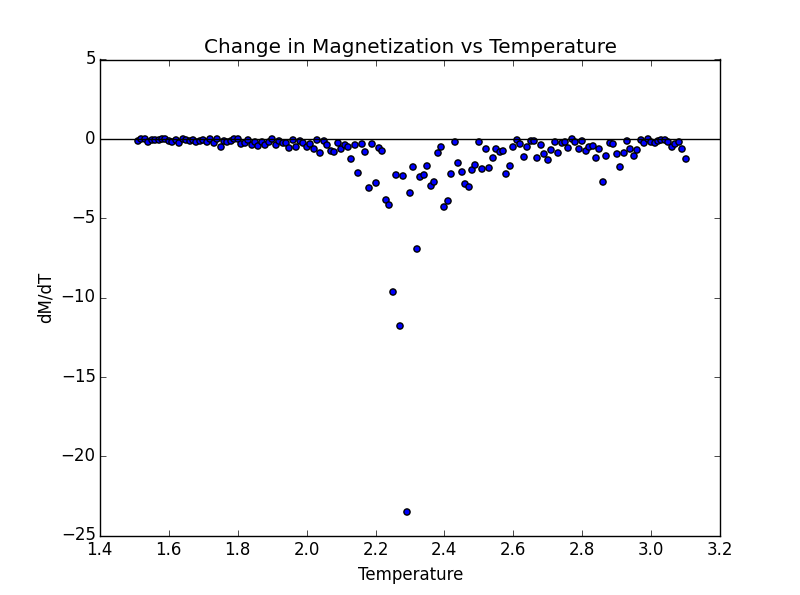
\includegraphics[scale=0.5]{Figures/dMdT.png}
\caption{Susceptibility of a 100x100 lattice. The peak/trough occurs at T = 2.28}
\label{fig:dMdT}
\end{figure} 

\noindent Looking at $T > 2.4$, we can see that the points vary to a more significant degree than the points less than 2.1. We found it increasingly difficult with larger and larger lattice sizes to keep the noise down at higher temperatures. To achieve figure \ref{fig:dMdT} (our best result) we increased the number of cluster runs for higher temperatures. This was thought to be the best solution because at higher temperatures the clusters do not grow very large (or at all) and we need to make sure to sample all the cells. So if the lattice is of size N=100. Then there are $100^2$=10,000 cells to sample. To be sure each lattice had entered a \textit{steady state} before we sampled the magnetization and internal energy, we used $2*N^2$ clusters for higher temperatures.
 
\subsection{Internal Energy}
The most energetically favorable state is when all cells have spins up and down in equal numbers.  This is why the graph of internal energy, figure \ref{fig:energy2}, looks like a mirrored version of the graph of magnetization, figure \ref{fig:Mag}. 

\begin{figure}[h]
\centering
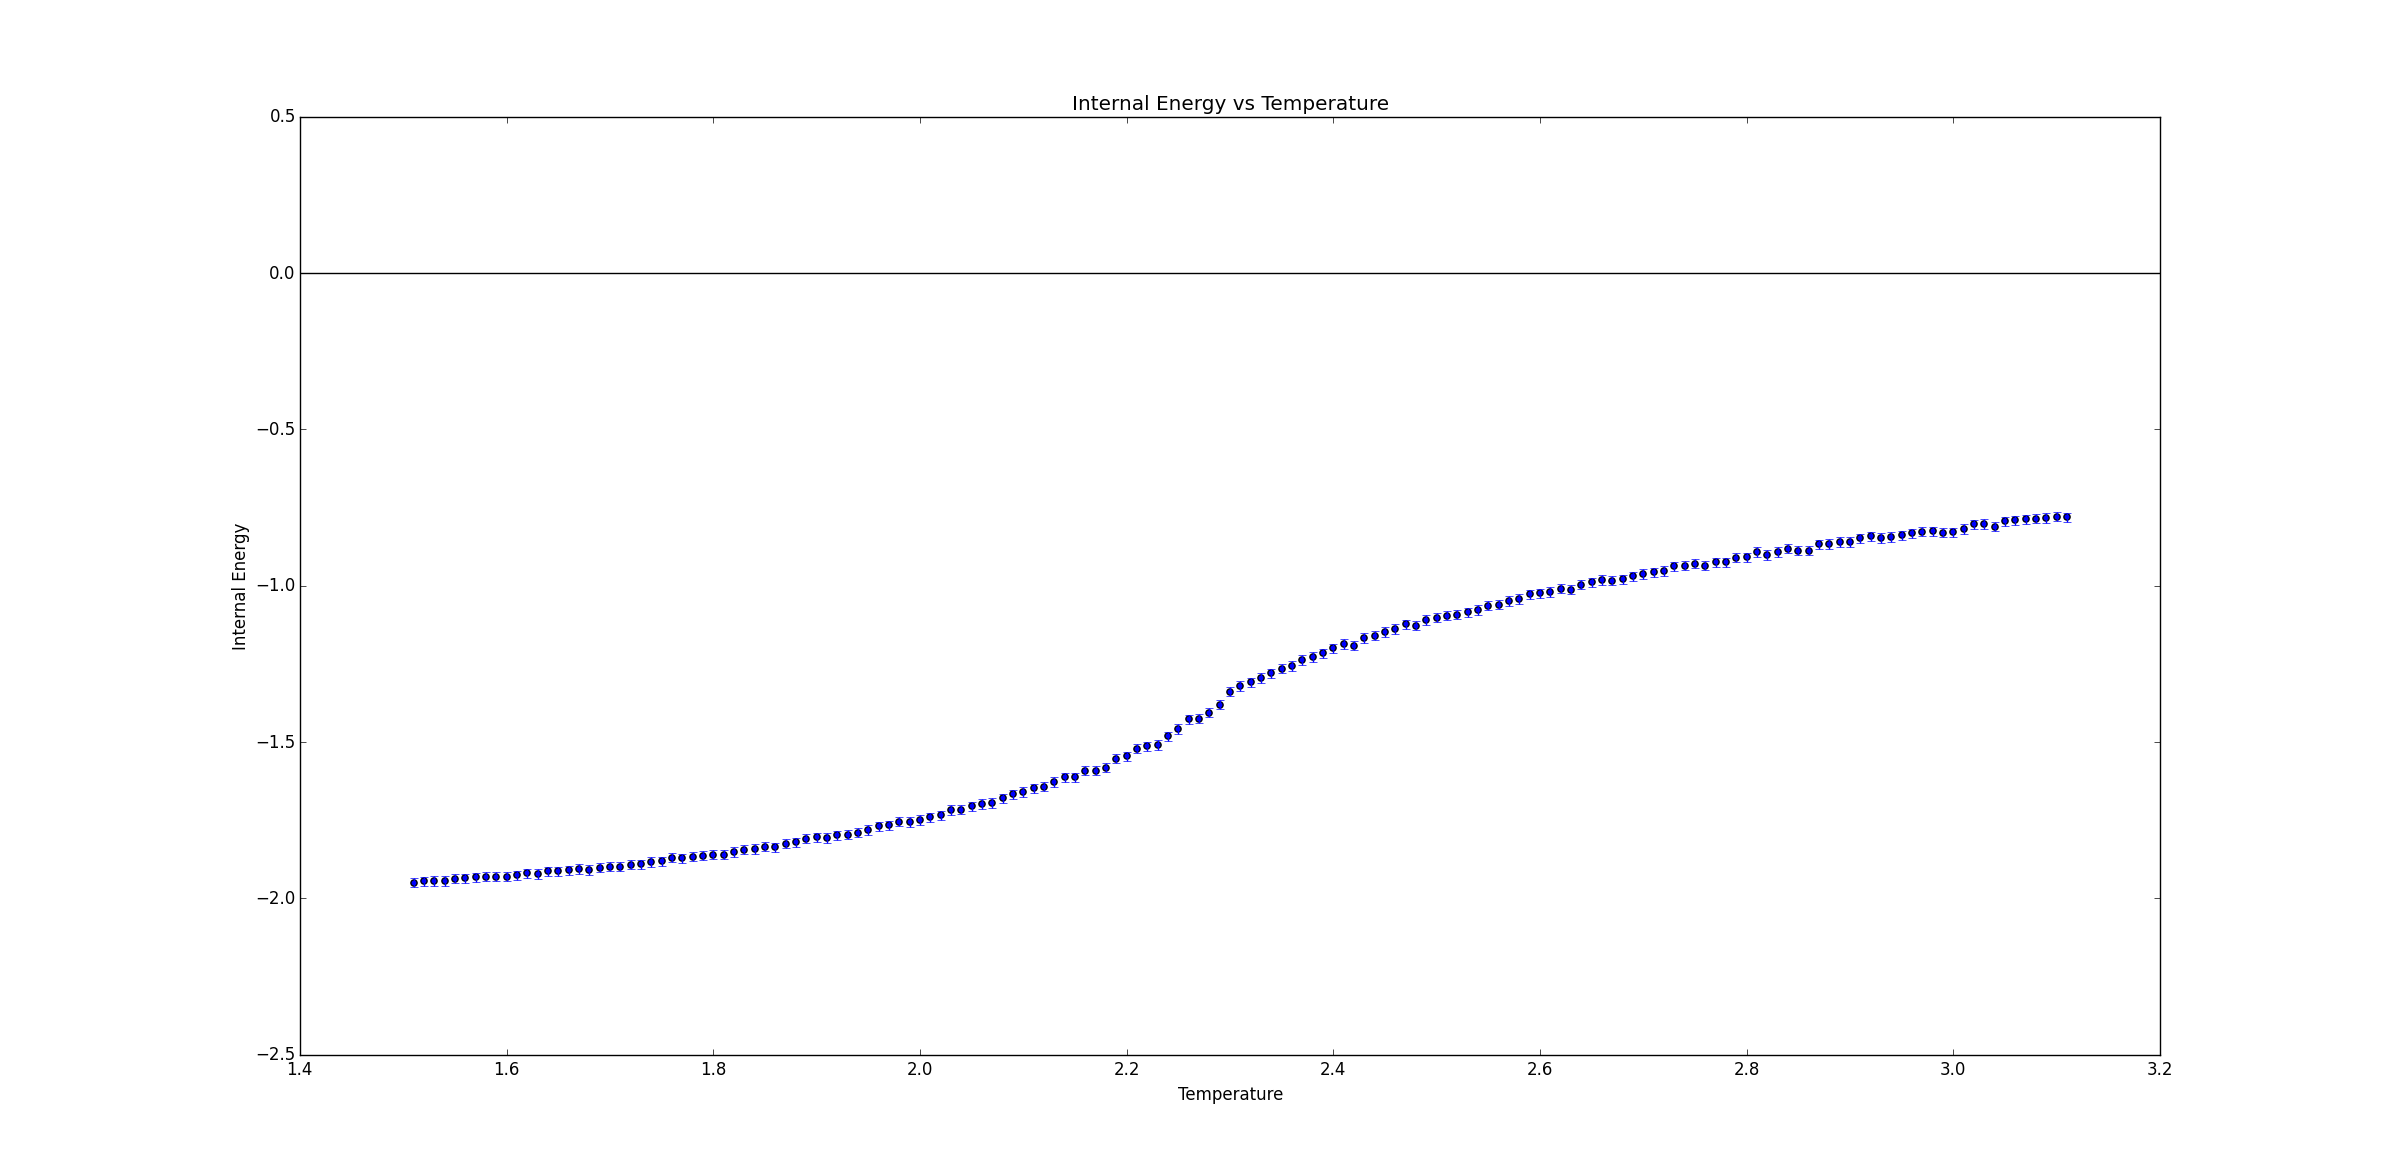
\includegraphics[scale=0.2]{Figures/energy2.png}
\caption{Internal Energy of 100x100 lattice}
\label{fig:energy2}
\end{figure} 

\noindent We calculated the internal energy of the system using equation \ref{eq:energy}.

\begin{equation}
\label{eq:energy}
E_{j} = -J\sum_{i} S_{i}S_{j}
\end{equation}

\noindent The energy of each cell, $E_{j}$, was calculated by summing the spin of that cell, $S_{j}$, with the spins of its neighbors, $S_{i}$. The total internal energy could then be calculated from this. The problem was not to double count a connection which you have already done before. The trick was to only sum the neighbors for the top and right, starting in the lower left corner. This ensured that every connection was accounted for with no double counting.

\subsection{Specific Heat}
The change in internal energy, figure \ref{fig:dEdT}, has a noisy, but notable peak around the critical temperature. This makes sense because we see a sudden increase in the internal energy from figure \ref{fig:energy2} around that point as well. 

\begin{figure}[h]
\centering
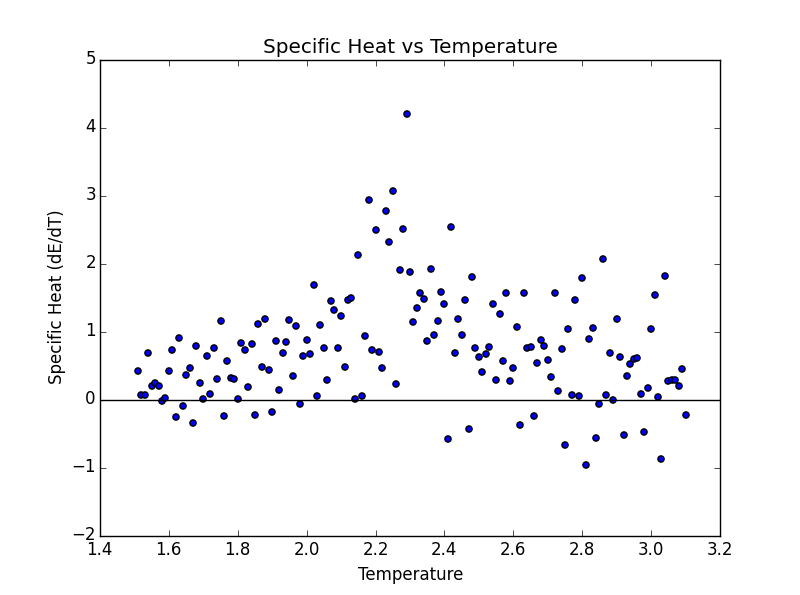
\includegraphics[scale=0.5]{Figures/dEdT.png}
\caption{Specific Heat of a 100x100 lattice, notable peak around critical temperature}
\label{fig:dEdT}
\end{figure} 

\noindent This change in internal energy is also the specific heat of the lattice. This shows that the change in energy needed for the temperature to increase is most dynamic around the critical temperature.

\subsection{Value of Gamma}

\begin{figure}[h]
\centering
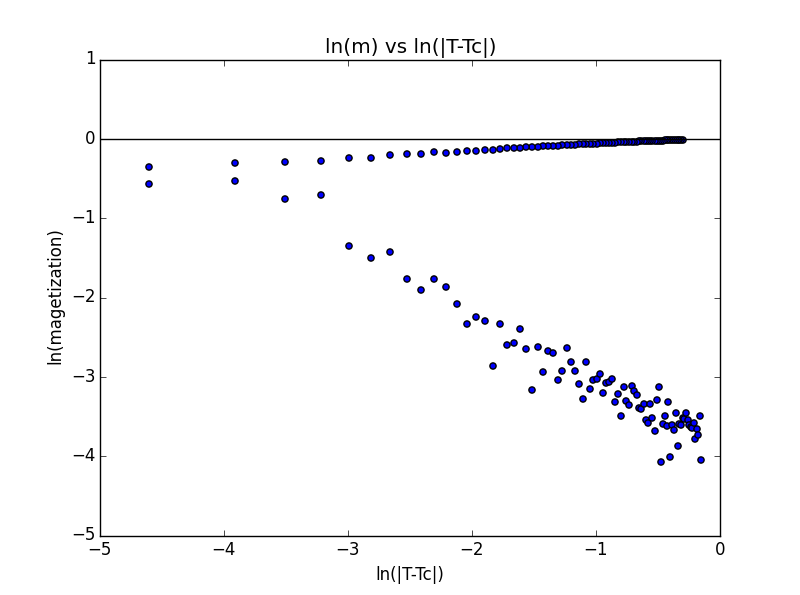
\includegraphics[scale=0.5]{Figures/gamma.png}
\caption{Plotting ln(m) v ln(|T-Tc|) for 1.5< T <3.1}
\label{fig:gamma}
\end{figure} 

\begin{figure}[h]
\centering
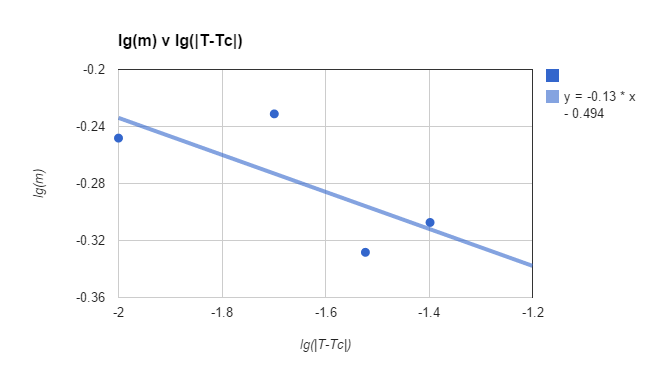
\includegraphics[scale=0.7]{Figures/gamma2.png}
\caption{Plotting ln(m) v ln( abs( T-Tc ) ) for 2.25$<$ T $<$2.291; Tc = 2.28}
\label{fig:gamma2}
\end{figure} 

\noindent Figures \ref{fig:gamma} and \ref{fig:gamma2} shown above are both log-log plots of magnetization and temperature. The idea behind this is to take the difference between the variable T and the fixed critical temperature, $T_{c}$, and plot it against the magnetization on a log-log plot to find the value of $\gamma$ in equation \ref{eq:gamma}. The slope of a linear line on a log-log plot is the value of the dependent variable's exponent. Seen in equation \ref{eq:gamma2}

\begin{equation}
\label{eq:gamma}
m = |{T-T_{c}}|^{\gamma}
\end{equation}

\begin{equation}
\label{eq:gamma2}
lg(m) = \gamma * lg(|{T-T_{c}}|)
\end{equation}


\noindent This task proved more difficult than originally thought. The top plot, figure \ref{fig:gamma}, is graphed over the whole range of temperatures which the program ran. We zoomed into just after the critical temperature in hopes of find $\gamma$. However, I find this whole process sketchy. Although I managed to fit the data in figure \ref{fig:gamma2} to give a slope which approximates the expected value of $\gamma$ ($1/8^{th}$), it felt force. I also expected $\gamma$ to turn out positive, however, that was not the case. I suspect that something is wrong in the way we calculated the value, based on the fact that our other graphs resemble what we expected, however, the source of the discrepancy is still being sought. 

\section{Conclusions and Discussion}
The ability to apply Monte Carlo Methods to physics problems has many applications. From this assignment here, we saw how it could be used to solve the Ising Model. From random sampling and the probabilistic growth of clusters within a magnetic lattice we were able to deduce the critical temperature to a reasonable certainty. 

\vspace{3mm}

\noindent Several questions and some confusion arose from working on this project. Particularly with the calculations of specific heat and $\gamma$.  One thing that did not make much sense was why the graph of internal energy, figure \ref{fig:energy2}, does not approach zero at the same temperature figure \ref{fig:Mag} does. It makes sense that if all spins are up and down in equal numbers the magnetization would be zero, but we wondered why the internal energy does not follow the same trend. Presumably, zero internal energy would be the most energetically favorable state. Perhaps the program must be run for longer and higher temperatures before the energy reaches zero, or maybe the energy calculations are flawed in someway which has yet to be found. The $\gamma$ calculations were very slow to move through as well. The calculations seemed relatively straight forward, however, extracting meaningful data from what came out seemed more trouble than expected. A possible improvement could be to run the simulations for more repetitions to reduce noise and refine the value of $T_{c}$.



\end{document}







